\documentclass[border=4pt]{standalone}
\usepackage{amsmath,amssymb}
\usepackage{tikz}
\usetikzlibrary{positioning,arrows.meta}
\newcommand{\add}{\boxplus}
\begin{document}
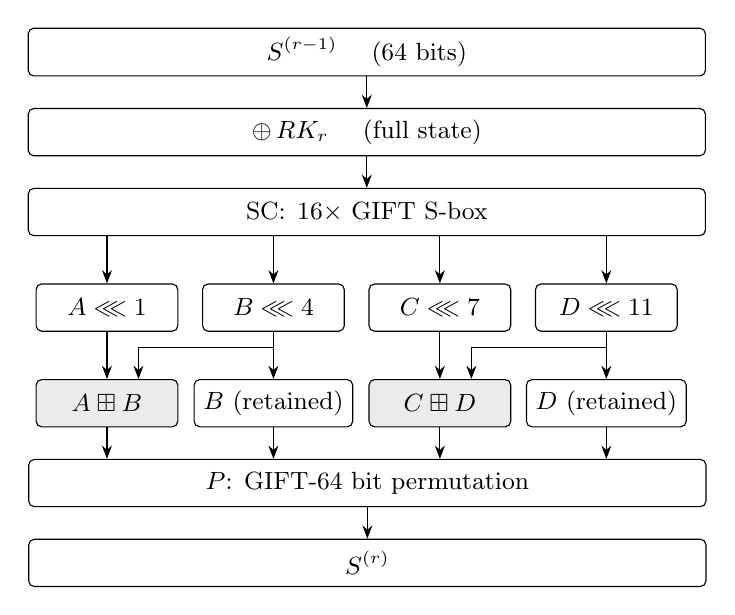
\begin{tikzpicture}[font=\small, >=Stealth,
  box/.style={draw, rounded corners=2pt, minimum height=6mm, align=center},
  w/.style={minimum width=18mm}]
\node[box, minimum width=86mm] (in) at (0,0) {$S^{(r-1)}$ \quad (64 bits)};
\node[box, minimum width=86mm, below=4mm of in] (ak) {$\oplus\,RK_r$ \quad (full state)};
\node[box, minimum width=86mm, below=4mm of ak] (sc) {$\mathrm{SC}$: $16\times$ GIFT S-box};
\node[box, w, below=6mm of sc.south west, anchor=north west, xshift=1mm] (a) {$A\lll1$};
\node[box, w, right=3mm of a] (b) {$B\lll4$};
\node[box, w, right=3mm of b] (c) {$C\lll7$};
\node[box, w, right=3mm of c] (d) {$D\lll11$};
\node[box, w, below=6mm of a, fill=black!8] (aa) {$A\add B$};
\node[box, w, below=6mm of b] (bb) {$B$ (retained)};
\node[box, w, below=6mm of c, fill=black!8] (cc) {$C\add D$};
\node[box, w, below=6mm of d] (dd) {$D$ (retained)};
\node[box, minimum width=86mm, below=4mm of bb.south west, anchor=north west, xshift=-21mm] (p) {$P$: GIFT-64 bit permutation};
\node[box, minimum width=86mm, below=4mm of p] (out) {$S^{(r)}$};
\draw[->] (in) -- (ak); \draw[->] (ak) -- (sc);
\foreach \x in {a,b,c,d} \draw[->] (sc.south -| \x.north) -- (\x.north);
\draw[->] (a) -- (aa); \draw[->] (b) -- (bb); \draw[->] (c) -- (cc); \draw[->] (d) -- (dd);
\draw[->] (b.south) -- ++(0,-2mm) -| ([xshift=4mm]aa.north);
\draw[->] (d.south) -- ++(0,-2mm) -| ([xshift=4mm]cc.north);
\foreach \x in {aa,bb,cc,dd} \draw[->] (\x.south) -- (p.north -| \x.south);
\draw[->] (p) -- (out);
\end{tikzpicture}
\end{document}
